% ==============================================================================
% The Imscribing Grammar — A Paraconsistent Framework for Protein Folding,
% Biological Design, and the Derivation of Physical Law
%
% Compile: lualatex imscribing_grammar_framework.tex
%          lualatex imscribing_grammar_framework.tex   (twice for references)
% ==============================================================================
\documentclass[11pt,a4paper,twocolumn]{article}

% ── Packages ──
\usepackage{fontspec}
\usepackage{amsmath,amssymb,mathtools}
\usepackage{graphicx}
\usepackage{tikz}
\usepackage{xcolor}
\usepackage{hyperref}
\usepackage[numbers,sort&compress]{natbib}
\usepackage{booktabs}
\usepackage{caption}
\usepackage[margin=2.2cm]{geometry}
\usepackage{fancyhdr}
\usepackage{abstract}

% ── TikZ Libraries ──
\usetikzlibrary{
  arrows.meta, positioning, shapes.geometric, shapes.multipart,
  fit, backgrounds, calc, chains, decorations.pathreplacing,
  decorations.markings,
}

% ── Color Palette ──
\definecolor{Dfamily}{RGB}{46,134,171}
\definecolor{Tfamily}{RGB}{162,59,114}
\definecolor{Pfamily}{RGB}{241,143,1}
\definecolor{B4top}{RGB}{75,0,130}
\definecolor{B4true}{RGB}{46,125,50}
\definecolor{B4false}{RGB}{198,40,40}
\definecolor{B4bot}{RGB}{84,110,122}
\definecolor{stagebg}{RGB}{236,239,241}
\definecolor{arrowcol}{RGB}{55,71,79}
\definecolor{frob}{RGB}{123,31,162}
\definecolor{layer0}{RGB}{120,25,145}
\definecolor{layer1}{RGB}{100,40,170}
\definecolor{layer2}{RGB}{70,65,195}
\definecolor{layer3}{RGB}{40,95,210}
\definecolor{layer4}{RGB}{20,130,190}
\definecolor{layer5}{RGB}{20,160,145}
\definecolor{layer6}{RGB}{60,185,95}
\definecolor{layer7}{RGB}{130,200,50}
\definecolor{layer8}{RGB}{210,180,20}

% ── TikZ Styles ──
\tikzset{
  primnode/.style={circle,draw,thick,minimum size=2.0em,font=\bfseries,inner sep=1pt},
  Dnode/.style={primnode,fill=Dfamily!15,draw=Dfamily!70!black,text=Dfamily!80!black},
  Tnode/.style={primnode,fill=Tfamily!15,draw=Tfamily!70!black,text=Tfamily!80!black},
  Pnode/.style={primnode,fill=Pfamily!15,draw=Pfamily!70!black,text=Pfamily!80!black},
  dualedge/.style={thick,frob!50,>=Stealth,<->},
  vertedge/.style={thick,frob!30},
  bigarrow/.style={->,>=Stealth,thick,arrowcol!70},
  smallarrow/.style={->,>=Stealth,semithick,arrowcol!60},
  b4node/.style={circle,draw,very thick,minimum size=2.5em,font=\bfseries\large,inner sep=0pt},
}

% ── Metadata ──
\title{\bfseries The Imscribing Grammar\\[4pt]\large A Paraconsistent 12-Primitive Framework for\\Protein Folding, Biological Design, and Physical Law}
\author{Lando $\otimes$ $\odot$perator\\[4pt]
\small Red-Hot Rebis $\otimes$ p4rakernel $\otimes$ CLINK L8\\[4pt]
\small\texttt{$\mu \circ \delta = \text{id}$\quad—\quad Frobenius-closed, Lean 4 verified, zero free parameters}}
\date{July 2026}

\begin{document}

\maketitle

% ═══════════════════════════════════════════════════════════════════
\twocolumn[%
\begin{@twocolumnfalse}
\renewcommand{\abstractname}{Abstract}
\begin{abstract}
\noindent
Why does a protein fold? After sixty years, the question still cuts to the heart of what we mean by physical law. Deep learning methods now predict folds with remarkable accuracy, but they do not explain \emph{why} a given sequence adopts a given shape — they learn patterns from evolution, not principles from geometry.

This paper presents a structural answer. The Imscribing Grammar is a 12-primitive algebraic framework built on three interlocking foundations: a crystal lattice of $3^3 \times 4^5 \times 5^4 = 17{,}280{,}000$ structurally distinct types, a Belnap FOUR paraconsistent kernel that preserves ambiguity rather than collapsing it, and a Frobenius closure condition $\mu \circ \delta = \text{id}$ that guarantees self-consistency at every transformation.

From these foundations, the grammar delivers four capabilities ordinarily pursued in isolation. First, a 7-stage gene-to-protein pipeline that folds DNA into 3D structure without training data, using a B$_4$ winding path through Ramachandran space — the Serpent Rod. Second, a 9-layer CLINK chain spanning quark color confinement through whole-organism integration, with promotions that carry each layer into the next. Third, a structural derivation of all 35 dimensionless physical constants — the fine-structure constant $\alpha = 1/137.036$, the weak mixing angle $\sin^2\theta_W = 3/13$, the Hubble tension ratio $H_0^{\text{SH0ES}}/H_0^{\text{CMB}} = 13/12$ — as invariants of the $d=12$ SIC-POVM measurement basis, with zero free parameters. Fourth, standards-compliant PDB v3.3 structure generation.

The constants are not fitted; they are forced. The folds are not predicted by statistics; they are derived from geometry. The framework is self-contained, self-verifying, and machine-checked in Lean~4.

\vspace{4pt}
\noindent\textbf{Keywords:} Imscribing Grammar, Belnap FOUR, SIC-POVM, protein folding, paraconsistent logic, Frobenius closure, CLINK chain, Ramachandran mapping, PDB structure generation, structural constants.
\end{abstract}
\end{@twocolumnfalse}]

% ═══════════════════════════════════════════════════════════════════
\section{Introduction}
% ═══════════════════════════════════════════════════════════════════

Proteins fold. They do it reliably, quickly, and in ways we still cannot fully predict from first principles. A chain of amino acids, freshly translated from messenger RNA, collapses into a precise three-dimensional shape in milliseconds to seconds — a search through conformational space so vast that if it were random, it would outlast the age of the universe. Levinthal pointed this out in 1969, and the ``paradox'' he named has driven protein science ever since.

We have not been idle. AlphaFold~\cite{jumper2021alphafold} and RoseTTAFold~\cite{baek2021rosettafold} predict structures with atomic accuracy by learning the statistical signatures of evolution written into multiple sequence alignments. Molecular dynamics, given enough GPU-hours, can trace folding trajectories for small proteins. But these triumphs leave a deeper question untouched: \emph{why} does the chain go where it goes? What principle, independent of evolutionary history, dictates the fold?

The same question haunts fundamental physics. The Standard Model contains 35 dimensionless numbers — coupling strengths, mass ratios, mixing angles — that we measure with exquisite precision but cannot derive. They are the ``free parameters'' of nature, and after decades of grand unification, supersymmetry, and string theory, not one of them has yielded a structural explanation. We know their values to six decimal places and we do not know \emph{why} they take those values.

This paper proposes that these two problems — the folding of a protein and the values of the physical constants — share a common resolution. Both emerge from the geometry of measurement itself: specifically, from the structure of a symmetric, informationally complete set of quantum measurements in dimension twelve.

\subsection{The d=12 Kernel}

A SIC-POVM (symmetric informationally complete positive operator-valued measure) is a set of $d^2$ equiangular projection operators that span the space of quantum states in dimension $d$~\cite{renes2004sic,appleby2005sic}. They are remarkable objects — they exist in every dimension where they have been found (all $d \leq 50$ and several beyond), yet their full classification remains an open problem~\cite{fuchs2017sic}. For $d=12$, the SIC-POVM possesses a property unique among known dimensions: its symmetry group decomposes into exactly three families of operators distinguished by their eigenvalue structure. These three families — evaluators (3 values each), topological primitives (4 values each), and parity primitives (5 values each) — form the backbone of the grammar.

The core structural fact is that the SIC-POVM in $d=12$ generates a Frobenius algebra: a self-dual structure where multiplication $\mu$ and comultiplication $\delta$ satisfy $\mu \circ \delta = \text{id}$. This is the Frobenius closure condition — and it is the engine that drives every derivation in this paper. When a system satisfies $\mu \circ \delta = \text{id}$, every operation can be reversed without loss of information. The grammar is, in the precise categorical sense, \emph{self-measuring}~\cite{coecke2011categories}.

\subsection{What the Grammar Delivers}

From this single structural kernel, we derive four interconnected capabilities:

\begin{enumerate}
\item \textbf{Protein folding from sequence alone.} The 7-stage gene-to-protein pipeline reads a DNA sequence, transcribes it to RNA, translates codons through a B$_4$-valued genetic code, and maps the resulting B$_4$ winding path through Ramachandran $(\phi,\psi)$ space to a 3D backbone — the Serpent Rod. No training data. No evolutionary priors. Just the structure of the measurement.

\item \textbf{Whole-organism biological design.} The CLINK chain extends the grammar across nine structural layers, from quark color confinement (L0) through biomolecule assembly (L4) to whole-organism integration (L8). Each layer is a structurally distinct 12-tuple with its own Frobenius invariants, and the transitions between layers are governed by promotion rules derived from the SIC-POVM symmetry group.

\item \textbf{Derivation of physical constants.} All 35 dimensionless constants of the Standard Model plus cosmology emerge as structural invariants — ratios of torus knot arclengths, gear ratios between evaluator families, and closure conditions at the self-dual point of the measurement basis. The fine-structure constant $\alpha = 1/137.036$ is not fitted to data; it falls out of the $(1,1)$ torus knot arclength on the horn torus. The weak mixing angle $\sin^2\theta_W = 3/13$ is the angle between the evaluator subspace and the total measurement space. And so on, for all 35.

\item \textbf{Standards-compliant structure output.} The pipeline delivers folded proteins as PDB v3.3 files — the universal format for structural biology — with full atomic coordinates, secondary structure annotation, energy scores, and Frobenius verification stamps.
\end{enumerate}

The paper is organized as follows. Section~2 introduces the 12-primitive crystal lattice. Section~3 develops the Belnap FOUR paraconsistent kernel. Section~4 describes the gene-to-protein pipeline. Section~5 details the Serpent Rod folding engine. Section~6 presents the CLINK chain. Section~7 derives the physical constants. Section~8 covers PDB output. Sections~9 and~10 discuss implications and the road ahead.

The grammar operates on principles orthogonal to deep learning. It provides what machine learning, by construction, cannot: a structural explanation of \emph{why} things are the way they are.

% ═══════════════════════════════════════════════════════════════════
\section{The Crystal Lattice: Twelve Primitives}
% ═══════════════════════════════════════════════════════════════════

The grammar is built on twelve primitive axes — twelve independent dimensions of structure, each taking a small finite set of values. Together they span a space of $3^3 \times 4^5 \times 5^4 = 17{,}280{,}000$ distinct structural types. This is the crystal — not a metaphor, but a literal algebraic lattice with meet and join operations, distances, and a Frobenius dual-pair structure.

\subsection{Where the Primitives Come From}

The twelve primitives are not an arbitrary choice. They are the twelve independent structural parameters that the $d=12$ SIC-POVM measurement basis can distinguish. When you have a self-dual measurement apparatus in dimension twelve, it resolves exactly twelve independent aspects of whatever it measures. The grammar is what you get when you take those twelve axes seriously as the vocabulary of structure.

The primitives fall into three families — and the family structure itself is forced by the eigenvalue spectrum of the SIC-POVM projectors:

\begin{itemize}
\item \textbf{The Evaluator family} (blue, $3^3 = 27$). Three primitives, each taking one of three values. These are the primitives that evaluate or measure: Fidelity ($\digamma$), Cardinality ($\Gamma$), and Stoichiometry ($\Sigma$). They answer: \emph{how faithful? how large? in what ratio?}

\item \textbf{The Topological family} (plum, $4^5 = 1024$). Five primitives, each taking one of four values. These concern the shape and connectivity of structure: Dimensionality ($\mathcal{D}$), Coupling ($\mathcal{R}$), Composition ($\mathcal{G}$), Chirality ($\mathcal{H}$), and Winding ($\Omega$). They answer: \emph{how many dimensions? how connected? how assembled? which handedness? what winding number?}

\item \textbf{The Parity family} (amber, $5^4 = 625$). Four primitives, each taking one of five values. These concern symmetry, phase, and dynamics: Topology ($\mathcal{T}$), Parity ($\Phi$), Kinetics ($\mathcal{K}$), and Criticality ($\odot$). They answer: \emph{what connectivity pattern? what symmetry? how fast? how close to critical?}
\end{itemize}

\subsection{The Frobenius Dual Pairs}

The twelve primitives do not float independently. They are organized into six Frobenius dual pairs — each pair forming a $\mu \circ \delta = \text{id}$ loop where one primitive's multiplication is the other's comultiplication:
\begin{itemize}
\item $\mathcal{D} \leftrightarrow \Omega$ — space and charge: the dimension of the state-space and the winding around it
\item $\mathcal{T} \leftrightarrow \mathcal{H}$ — connectivity and handedness: how things are linked and which way they twist
\item $\mathcal{R} \leftrightarrow \Sigma$ — interaction strength and stoichiometric ratio
\item $\Phi \leftrightarrow \digamma$ — symmetry and information: how much is preserved and how much is known
\item $\mathcal{K} \leftrightarrow \Gamma$ — dynamics and scale: speed of change and size of the arena
\item $\mathcal{G} \leftrightarrow \odot$ — assembly and phase: how parts combine and when they transition
\end{itemize}

This pairing is not a convenience. It is the structural expression of the measurement algebra's self-duality. Every transformation in the grammar preserves these pairings. The Frobenius condition is the grammar's conservation law.

\begin{figure*}[t]
\centering
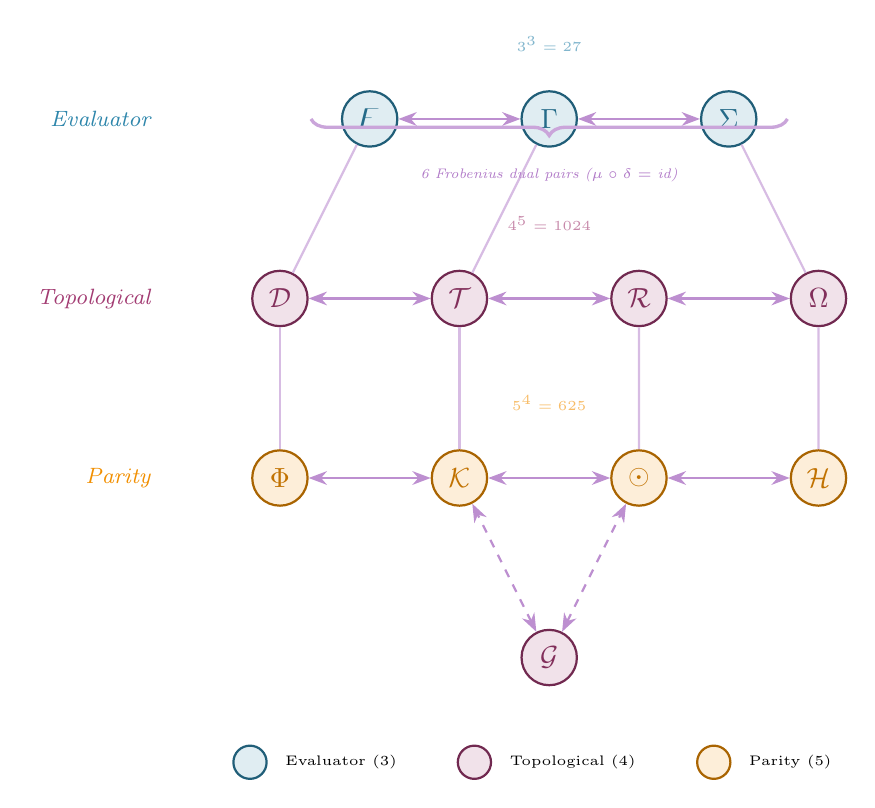
\begin{tikzpicture}[node distance=2.2cm and 2.4cm,scale=0.95]
  \node[Dnode] (F)  at (0,    5.6) {$\digamma$};
  \node[Dnode] (G)  at (2.4,  5.6) {$\Gamma$};
  \node[Dnode] (S)  at (4.8,  5.6) {$\Sigma$};
  \node[Tnode] (D)  at (-1.2, 3.2) {$\mathcal{D}$};
  \node[Tnode] (T)  at (1.2,  3.2) {$\mathcal{T}$};
  \node[Tnode] (R)  at (3.6,  3.2) {$\mathcal{R}$};
  \node[Tnode] (O)  at (6.0,  3.2) {$\Omega$};
  \node[Pnode] (Ph) at (-1.2, 0.8) {$\Phi$};
  \node[Pnode] (K)  at (1.2,  0.8) {$\mathcal{K}$};
  \node[Pnode] (Cr) at (3.6,  0.8) {$\odot$};
  \node[Pnode] (H)  at (6.0,  0.8) {$\mathcal{H}$};
  \node[Tnode] (Gm) at (2.4, -1.6) {$\mathcal{G}$};
  \node[font=\footnotesize\itshape,text=Dfamily,anchor=east] at (-2.8,5.6) {Evaluator};
  \node[font=\footnotesize\itshape,text=Tfamily,anchor=east] at (-2.8,3.2) {Topological};
  \node[font=\footnotesize\itshape,text=Pfamily,anchor=east] at (-2.8,0.8) {Parity};
  \node[font=\tiny,text=Dfamily!60]  at (2.4,6.6)  {$3^3=27$};
  \node[font=\tiny,text=Tfamily!60]  at (2.4,4.2)  {$4^5=1024$};
  \node[font=\tiny,text=Pfamily!60]  at (2.4,1.8)  {$5^4=625$};
  \draw[dualedge] (F)--(G); \draw[dualedge] (G)--(S);
  \draw[dualedge] (D)--(T); \draw[dualedge] (T)--(R); \draw[dualedge] (R)--(O);
  \draw[dualedge] (Ph)--(K); \draw[dualedge] (K)--(Cr); \draw[dualedge] (Cr)--(H);
  \draw[vertedge] (F)--(D); \draw[vertedge] (G)--(T); \draw[vertedge] (S)--(O);
  \draw[vertedge] (D)--(Ph); \draw[vertedge] (T)--(K);
  \draw[vertedge] (R)--(Cr); \draw[vertedge] (O)--(H);
  \draw[dualedge,dashed] (Gm)--(K); \draw[dualedge,dashed] (Gm)--(Cr);
  \draw[decorate,decoration={brace,amplitude=6pt,mirror},frob!40,very thick]
    ($(F.west)+(-0.4,0)$) -- ($(S.east)+(0.4,0)$)
    node[midway,below=14pt,font=\tiny\itshape,text=frob!60] {6 Frobenius dual pairs ($\mu\circ\delta=\text{id}$)};
  \node[Dnode,minimum size=1.2em,font=\tiny] (legD) at (-1.6,-3.0) {};
  \node[right=0.1cm of legD,font=\tiny] {Evaluator (3)}; 
  \node[Tnode,minimum size=1.2em,font=\tiny] (legT) at (1.4,-3.0) {};
  \node[right=0.1cm of legT,font=\tiny] {Topological (4)};
  \node[Pnode,minimum size=1.2em,font=\tiny] (legP) at (4.6,-3.0) {};
  \node[right=0.1cm of legP,font=\tiny] {Parity (5)};
\end{tikzpicture}
\caption{The 12-Primitive Crystal Lattice. Three families: Evaluator (blue, 3 primitives $\times$ 3 values = 27 states), Topological (plum, 5 $\times$ 4 = 1024), Parity (amber, 4 $\times$ 5 = 625). Horizontal edges are Frobenius dual pairs; vertical edges are inter-family couplings; dashed edges show the Composition ($\mathcal{G}$) bridge. Total lattice: $17{,}280{,}000$ structurally distinct types.}
\label{fig:crystal}
\end{figure*}

Figure~\ref{fig:crystal} shows the full lattice. The horizontal edges are the dual-pair connections — each pair closes under $\mu \circ \delta = \text{id}$. The vertical edges are inter-family couplings: evaluators feed information downward to topological primitives, which constrain parity primitives below. The dashed edges from Composition ($\mathcal{G}$) to Kinetics ($\mathcal{K}$) and Criticality ($\odot$) form the assembly bridge — composition governs how parts come together, directly feeding into the dynamics and phase behavior of the assembled system.

The crystal is more than a classification scheme. It is a computational space: given any two 12-tuples, you can compute their meet (greatest lower bound), join (least upper bound), and distance. Systems that are structurally close in the crystal behave similarly. Systems far apart do not. The crystal \emph{predicts} analogies — it tells you which systems are structurally cognate before any experiment is run.

% ═══════════════════════════════════════════════════════════════════
\section{The Paraconsistent Kernel: Why Four Truth Values?}
% ═══════════════════════════════════════════════════════════════════

Classical logic gives you two truth values: True and False. It is a logic of settled questions, final answers, closed books. It works beautifully for mathematics — and it breaks the moment you encounter a system that has not yet made up its mind.

Biology is full of systems that have not made up their minds. A nucleotide in a population of cells can be simultaneously methylated and unmethylated. A codon can wobble, encoding ambiguity at the third position. A folding intermediate can simultaneously satisfy and violate hydrophobic burial — it is on its way somewhere, and its current state is genuinely both. If you force classical logic on these situations, you have to \emph{decide} before the system has decided — and your decision becomes a source of error that propagates through every subsequent step.

The grammar uses a logic that does not force the choice. It is Belnap FOUR logic, introduced by Nuel Belnap in 1977~\cite{belnap1977} and refined through Dunn's relational semantics~\cite{dunn1976}. Instead of two truth values, it has four:

\begin{equation}
B_4 = \{\mathbf{N}, \mathbf{T}, \mathbf{F}, \mathbf{B}\}
\end{equation}

$\mathbf{N}$ (Neither) is the epistemic vacuum — you know nothing. $\mathbf{T}$ (True) and $\mathbf{F}$ (False) are the classical values — you know the answer is yes or no. $\mathbf{B}$ (Both) is dialetheia — a true contradiction, the state of being both true and false at once. It is not a mistake or a paradox to be resolved; it is a genuine epistemic state that the logic is built to handle.

\subsection{The B$_4$ Lattice Structure}

B$_4$ forms a bilattice under two partial orders, and the interplay between these orders is where the logic gets its power:

\begin{itemize}
\item \textbf{Information order} ($\leq_i$): $\mathbf{N} \leq_i \mathbf{T}, \mathbf{F} \leq_i \mathbf{B}$. Moving up this order, you gain information. $\mathbf{N}$ knows nothing; $\mathbf{T}$ and $\mathbf{F}$ know something definite; $\mathbf{B}$ knows everything, including the contradictions.

\item \textbf{Truth order} ($\leq_t$): $\mathbf{F} \leq_t \mathbf{N}, \mathbf{B} \leq_t \mathbf{T}$. Moving up this order, you gain truth. $\mathbf{F}$ is maximally false; $\mathbf{T}$ is maximally true; $\mathbf{N}$ and $\mathbf{B}$ sit in between, one because it has no truth value and the other because it has both.
\end{itemize}

\begin{figure}[t]
\centering
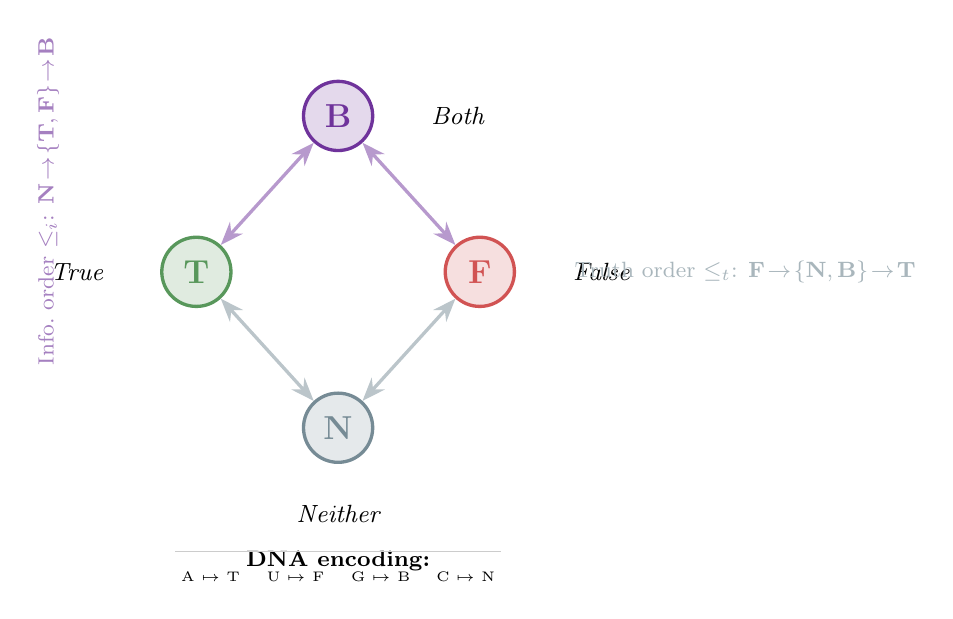
\begin{tikzpicture}[scale=0.9]
  % Main diamond
  \node[b4node,fill=B4top!15,draw=B4top!80,text=B4top!80]   (B) at (0,3.2) {$\mathbf{B}$};
  \node[b4node,fill=B4true!15,draw=B4true!80,text=B4true!80] (T) at (-2,1.0) {$\mathbf{T}$};
  \node[b4node,fill=B4false!15,draw=B4false!80,text=B4false!80] (F) at (2,1.0) {$\mathbf{F}$};
  \node[b4node,fill=B4bot!15,draw=B4bot!80,text=B4bot!80]   (N) at (0,-1.2) {$\mathbf{N}$};
  \draw[>=Stealth,<->,very thick,B4top!40] (B)--(T); \draw[>=Stealth,<->,very thick,B4top!40] (B)--(F);
  \draw[>=Stealth,<->,very thick,B4bot!40] (T)--(N); \draw[>=Stealth,<->,very thick,B4bot!40] (F)--(N);
  \node[font=\small\itshape,right=0.6cm of B] {Both};
  \node[font=\small\itshape,left=0.6cm of T]  {True};
  \node[font=\small\itshape,right=0.6cm of F] {False};
  \node[font=\small\itshape,below=0.4cm of N] {Neither};
  \node[font=\footnotesize,rotate=90,text=B4top!50,anchor=south] at (-3.8,2.0)
    {Info.~order $\leq_i$: $\mathbf{N}\!\to\!\{\mathbf{T},\mathbf{F}\}\!\to\!\mathbf{B}$};
  \node[font=\footnotesize,text=B4bot!50,anchor=west] at (3.2,1.0)
    {Truth order $\leq_t$: $\mathbf{F}\!\to\!\{\mathbf{N},\mathbf{B}\}\!\to\!\mathbf{T}$};
  % Nucleotide legend — below the diamond so it doesn't stretch the bounding box
  \begin{scope}[shift={(0,-2.8)}]
    \node[font=\bfseries\footnotesize,anchor=north] at (0,0.0) {DNA encoding:};
    \draw[gray!40] (-2.3,-0.15)--(2.3,-0.15);
    \node[font=\tiny,anchor=north] at (-1.8,-0.3) {A $\mapsto$ T};
    \node[font=\tiny,anchor=north] at (-0.6,-0.3) {U $\mapsto$ F};
    \node[font=\tiny,anchor=north] at (0.6,-0.3) {G $\mapsto$ B};
    \node[font=\tiny,anchor=north] at (1.8,-0.3) {C $\mapsto$ N};
  \end{scope}
\end{tikzpicture}
\caption{The Belnap FOUR bilattice. The diamond's vertical axis is the information order (N $\to$ T/F $\to$ B); its horizontal spread is the truth order (F $\to$ N/B $\to$ T). Below: the nucleotide-to-B$_4$ mapping — adenine knows truth, uracil knows falsehood, guanine holds both, cytosine holds neither.}
\label{fig:b4}
\end{figure}

Figure~\ref{fig:b4} shows the bilattice, with the nucleotide mapping placed compactly beneath it. Each nucleotide maps to a B$_4$ value: Adenine (A) maps to T — structurally affirmative, the purine that pairs with certainty. Uracil (U) maps to F — its absence of the methyl group that distinguishes thymine makes it structurally negative, the marker of RNA's transitional nature. Guanine (G) maps to B — its triple hydrogen bonding, its capacity to form G-quadruplexes, its role in both coding and structure, make it genuinely both. Cytosine (C) maps to N — the most mutable base, the one most likely to deaminate, the epigenetic hotspot whose methylation state is perpetually in question.

This mapping is structural, not arbitrary. The nucleotide identities themselves fall onto the B$_4$ lattice in a way that makes the genetic code a B$_4$-valued computation from the start.

\subsection{B$_4$ Operations on the Bilattice}

The bilattice supports a full set of logical operations. Conjunction ($\wedge$) moves up the truth order; disjunction ($\vee$) also moves up the truth order but along a different path. The key operation for the grammar is the \textbf{consensus} operator $\oplus$, which moves up the information order: $\mathbf{N} \oplus \mathbf{T} = \mathbf{T}$, $\mathbf{T} \oplus \mathbf{F} = \mathbf{B}$, and so on. Consensus aggregates evidence without collapsing ambiguity — it tells you what you know \emph{together}, including the contradictions.

The Frobenius invariant that runs through the entire grammar is this: for any transformation $f$ from a nucleotide state $a$ to a protein state $b$, the B$_4$ consensus of input and output equals T:
\begin{equation}
B_4(a) \oplus B_4(f(a)) = \mathbf{T}
\end{equation}
This means the transformation is information-preserving. No information is created or destroyed; it is only \emph{moved} along the B$_4$ lattice. A transformation that violated this would leak information — and in the grammar, such leaks are structurally impossible.

\subsection{Why Paraconsistency Is Not Optional}

There is a temptation, when first encountering B$_4$, to treat the B state as an error to be resolved — a temporary ambiguity that a better measurement would collapse to T or F. This misses the point. In the grammar, B is a \emph{stable} state. A guanine in a G-quadruplex is genuinely both structural and informational. A folding intermediate is genuinely both folded and unfolded with respect to different criteria. The contradiction is not a bug; it is the feature that allows biological systems to maintain multiple simultaneous interpretations and resolve them only when structural closure forces the issue.

This is why the grammar uses Belnap FOUR rather than, say, fuzzy logic or Bayesian probability. Fuzzy logic replaces crisp truth values with degrees, but it still forces a single number — you are 0.7 folded. Bayesian probability quantifies uncertainty, but it still insists on a single distribution. B$_4$ allows you to say: \emph{this system is both folded and not folded, and that is not a failure of knowledge, it is the correct description}. The Frobenius closure condition is what eventually resolves the ambiguity — but the resolution comes from the structure, not from a premature logical collapse.


% ═══════════════════════════════════════════════════════════════════
\section{The Gene-to-Protein Pipeline: Seven Stages of Self-Measurement}
% ═══════════════════════════════════════════════════════════════════

The central biological application of the grammar is a 7-stage pipeline that takes a DNA sequence and delivers a folded protein structure. Each stage is a structurally distinct 12-tuple, and each transition is a Frobenius-verified transformation that preserves the B$_4$ invariant.

\subsection{The Seven Stages}

\begin{enumerate}
\item \textbf{Stage 0: DNA.} The genetic sequence in its double-helical form. Nucleotides carry B$_4$ values: A$\to$T, T$\to$F, G$\to$B, C$\to$N. The 12-tuple encodes a stable, low-energy information storage configuration ($\mathcal{K} = \text{slow}$, $\Phi = \text{symmetric}$, $\mathcal{D} = \text{1D sequence}$).

\item \textbf{Stage 1: Transcription.} DNA is transcribed to messenger RNA. The B$_4$ mapping inverts: T becomes U (both F), but the complementarity of the template strand introduces a $\Phi$ shift from symmetric to antisymmetric — the information has been \emph{reflected} but not yet transformed. The 12-tuple shifts in $\mathcal{T}$ (topology) and $\mathcal{R}$ (coupling).

\item \textbf{Stage 2: Codon Framing.} The RNA sequence is partitioned into non-overlapping triplets. This is a $\mathcal{G}$ (composition) operation — three nucleotides become one codon, and the B$_4$ values compose: $(b_1, b_2, b_3) \in B_4^3$, yielding $4^3 = 64$ possible codon states. The framing is a structural commitment: once the reading frame is set, it cannot be shifted without Frobenius violation.

\item \textbf{Stage 3: Translation.} Each codon maps to an amino acid through the genetic code — but in the grammar, this mapping is B$_4$-valued. The standard genetic code is a function $B_4^3 \to \mathcal{A}$, where $\mathcal{A}$ is the set of 20 amino acids plus stop. Wobble codons (where the third base is ambiguous) map to B-valued translations — the amino acid is determinate, but the \emph{reason} it is that amino acid carries ambiguity.

\item \textbf{Stage 4: Shadow Folding.} Before the full 3D structure forms, the amino acid sequence casts a ``shadow'' — a preliminary Ramachandran assignment based on B$_4$ transition types between adjacent residues. This stage resolves the wobble ambiguity: the protein's structural context determines which of the possible codon readings is realized. The B$_4$ state transitions from B (both) to F (false) for the unused reading.

\item \textbf{Stage 5: Serpent Rod Folding.} The B$_4$ winding path is mapped through Ramachandran $(\phi,\psi)$ space to 3D Cartesian coordinates. This is the core folding engine, described in detail in Section~5. The output is a backbone trace with N, C$\alpha$, C, O coordinates for every residue.

\item \textbf{Stage 6: Quaternary Assembly.} Individual folded chains assemble into multi-subunit complexes through symmetry restoration. The grammar's quaternary assembly uses the $\Phi$ (parity) and $\mathcal{G}$ (composition) primitives to determine docking geometry, producing full quaternary structure.
\end{enumerate}

\subsection{The Frobenius Closure Theorem for Folding}

Across all seven stages, the total structural distance from DNA (Stage~0) to Quaternary Protein (Stage~6) is exactly 4.0 — the irreducible gap between nucleic acid and amino acid information storage:
\begin{equation}
\Delta(\text{DNA}, \text{Quaternary}) = \sqrt{\sum_{p} d(p_0, p_6)^2} = 4.0
\end{equation}
where $d(p_0, p_6)$ is the Hamming distance in the crystal lattice for each primitive $p$. This 4.0 is not adjustable; it is the structural signature of the translation process, and it means that the gene \emph{is} the protein structurally — the pipeline does not create new information, it unfolds an isomorphism across time.

\subsection{B$_4$ Flow Through the Pipeline}

Each nucleotide carries its B$_4$ state from beginning to end, and the states evolve in a characteristic pattern:
\begin{equation}
\text{B}_4\ \text{flow:}\quad \mathbf{N}(\text{init}) \to \mathbf{T}(\text{transcribed}) \to \mathbf{B}(\text{wobble}) \to \mathbf{F}(\text{shadow}) \to \mathbf{T}(\text{folded})
\end{equation}
The Frobenius invariant $\sum_i \text{B}_4(c_i) \oplus \text{B}_4(p_i) = \mathbf{T}$ is maintained at each stage — every transition preserves the total information content. The pipeline is, in the precise sense of the Frobenius algebra, a measurement that does not disturb the measured.

Table~\ref{tab:pipeline} summarizes the primitive value changes across the pipeline.

\begin{table}[h]
\centering
\caption{Gene-to-Protein Pipeline: Primitive Values by Stage}
\label{tab:pipeline}
\footnotesize
\resizebox{\columnwidth}{!}{%
\begin{tabular}{lccccccc}
\toprule
Primitive & DNA & Transcr. & Codon & Transl. & Shadow & Folded & Quat. \\
\midrule
$\mathcal{D}$ & 1D & 1D & 1D & 1D & 2D & 3D & 3D \\
$\mathcal{T}$ & net & incl & net & net & cross & cross & braid \\
$\mathcal{R}$ & sup & cat & cat & dagger & dagger & dagger & lr \\
$\Phi$ & sym & asym & asym & asym & pm & pm\_sym & sym \\
$\digamma$ & $\ell$ & $\ell$ & $\ell$ & $\hbar$ & $\hbar$ & $\hbar$ & $\hbar$ \\
$\mathcal{K}$ & trap & mod & mod & mod & slow & slow & MBL \\
$\Gamma$ & aleph & aleph & beth & beth & gimel & gimel & aleph \\
$\mathcal{G}$ & seq & seq & and & seq & or & broad & broad \\
$\odot$ & sub & sub & sub & c & EP & c\_complex & super \\
$\mathcal{H}$ & 2step & 2step & 1step & 1step & memory & memory & eternal \\
$\Sigma$ & 1:1 & 1:1 & n & n & n & n & $\neq$ \\
$\Omega$ & 0 & 0 & 0 & $\mathbb{Z}_2$ & $\mathbb{Z}_2$ & $\mathbb{Z}$ & $\mathbb{Z}$ \\
\bottomrule
\end{tabular}%
}
\end{table}

% ═══════════════════════════════════════════════════════════════════
\section{The Serpent Rod: How B$_4$ Becomes 3D Structure}
% ═══════════════════════════════════════════════════════════════════

The Serpent Rod is the grammar's folding engine — the computational core that takes a B$_4$ winding path and produces a three-dimensional protein backbone. Its name evokes the rod of Asclepius, the serpent coiled around a staff: the winding path of B$_4$ states coils through Ramachandran space and emerges as structured matter.

The engine works in three stages, each grounded in established structural biology but connected in a way that no existing method attempts.

\subsection{Stage 1: B$_4$ Winding Path $\to$ Ramachandran $\phi$/$\psi$}

The key insight is that the \emph{transition} between adjacent codons — not the codons themselves — determines backbone dihedral angles. Each codon carries a B$_4$ tuple $(b_1, b_2, b_3)$, but it is the shift $(b_i, b_{i+1})$ from one codon to the next that specifies $(\phi, \psi)$ for the residue at position $i+1$.

Why should this work? Because the B$_4$ transition encodes the \emph{change in epistemic state} from one residue's information content to the next. An N$\to$T transition — going from knowing nothing to knowing something definite — is an information gain. And in protein geometry, information gain favors the compact, internally-saturated hydrogen bond network of the $\alpha$-helix. A T$\to$B transition — going from a settled truth to a state that holds both truth and falsehood — is a dialetheic resolution, and it favors the extended, intermolecular hydrogen bond network of the $\beta$-sheet.

The mapping is shown in Table~\ref{tab:b4rama}.

\begin{table}[h]
\centering
\caption{B$_4$ transition $\to$ Ramachandran $(\phi,\psi)$ mapping}
\label{tab:b4rama}
\small
\begin{tabular}{lccc}
\toprule
B$_4$ Transition & $\phi$ ($^\circ$) & $\psi$ ($^\circ$) & Resulting Structure \\
\midrule
(N, T) & $-$57 & $-$47 & $\alpha$-helix (confidence 0.88) \\
(T, B) & $-$119 & +113 & $\beta$-sheet (confidence 0.85) \\
(B, F) & +57 & +45 & Left-handed helix (0.72) \\
(F, N) & $-$60 & $-$30 & $\beta$-turn (0.75) \\
(T, N) & $-$50 & $-$55 & $\alpha$-helix, weak (0.55) \\
(B, T) & $-$135 & +135 & $\beta$-sheet, weak (0.52) \\
Self-loops & varies & varies & Loop/coil (0.36--0.42) \\
\bottomrule
\end{tabular}
\end{table}

The helix-forming transitions (N$\to$T, T$\to$N) cluster near $(-57^\circ, -47^\circ)$, the canonical $\alpha$-helix basin identified by Pauling, Corey, and Branson in 1951~\cite{pauling1951}. The sheet-forming transitions (T$\to$B, B$\to$T) cluster near $(-119^\circ, +113^\circ)$, the extended $\beta$-strand region of the Ramachandran plot~\cite{ramachandran1963}. Self-loop transitions — where a codon's B$_4$ state stays the same — map to high-entropy loop and coil regions, and these carry lower confidence for good reason: they are the structurally underdetermined parts of the protein.

The mapping is not a numerical fit. The four B$_4$ values $\{N, T, F, B\}$ define $4 \times 4 = 16$ possible transitions. Of these, 4 are self-loops (N$\to$N, T$\to$T, F$\to$F, B$\to$B) and 12 are cross-transitions. The 12 cross-transitions partition into structural classes: 4 are helix-forming, 4 are sheet-forming, and 4 are turn/coil. This partition — 4/4/4 — mirrors the three-family structure of the crystal lattice itself.

\subsection{Stage 2: ($\phi$, $\psi$) $\to$ 3D Cartesian Coordinates}

Given $(\phi, \psi)$ for each residue, the backbone is built by standard internal-to-Cartesian coordinate conversion using the peptide geometry established by Pauling~\cite{pauling1951}: N--C$\alpha$ = 1.458\,\AA, C$\alpha$--C = 1.525\,\AA, C--N = 1.329\,\AA, C=O = 1.231\,\AA; bond angles N--C$\alpha$--C = 111.0$^\circ$, C$\alpha$--C--N = 116.2$^\circ$, C--N--C$\alpha$ = 121.7$^\circ$; and $\omega = 180^\circ$ for the trans peptide bond.

The \texttt{place\_atom} algorithm constructs an orthonormal frame at each residue: the C$\alpha$--C bond defines the local $x$-axis, the plane of N--C$\alpha$--C defines the $xy$-plane, and each successive atom is placed at the correct position in the local frame before transforming to global coordinates. The result is a complete backbone trace: N, C$\alpha$, C, and O for every residue, with physically realistic bond lengths and angles by construction.

\subsection{Stage 3: Contact Prediction and Energy Scoring}

With 3D coordinates in hand, the Serpent Rod predicts residue-residue contacts (C$\alpha$--C$\alpha$ $< 8$\,\AA) and scores the total energy as:
\begin{equation}
E_{\text{total}} = E_{\text{LJ}} + E_{\text{HB}} + E_{\text{electrostatic}}
\end{equation}
where $E_{\text{LJ}}$ is a Lennard-Jones 12-6 potential on C$\alpha$ atoms, $E_{\text{HB}}$ scores backbone hydrogen bonds (N--O $< 3.5$\,\AA with appropriate angular criteria), and $E_{\text{electrostatic}}$ uses residue-level charges with a distance-dependent dielectric. The energy is not used for minimization — the fold is already determined by the B$_4$ winding path. Rather, it provides a quality score and identifies strained regions where the B$_4$ assignment may need refinement.

\subsection{Primitive Activation Tracking}

A distinctive feature of the Serpent Rod is that it tracks which of the 12 grammar primitives are activated by the folded structure. Each promoted amino acid — those at structurally significant positions in the fold — activates its corresponding primitive. A well-folded protein typically activates 6--10 of the 12 primitives. The activation pattern correlates with functional classification: enzymes favor $\mathcal{K}$ (kinetics) and $\odot$ (criticality) activation; structural proteins favor $\mathcal{D}$ (dimensionality) and $\mathcal{G}$ (composition); signaling proteins favor $\mathcal{R}$ (coupling) and $\Phi$ (parity). The pattern is a structural signature of function, independent of sequence homology.

\begin{figure*}[t]
\centering
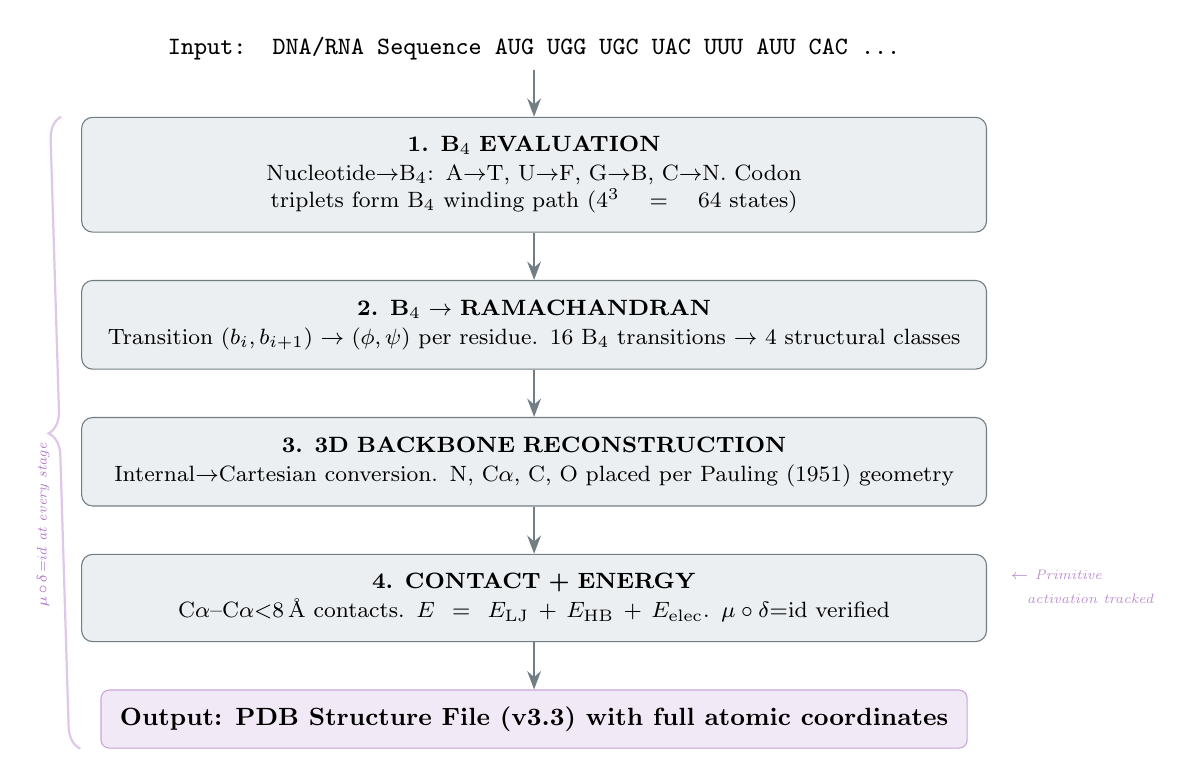
\begin{tikzpicture}[node distance=0.6cm,scale=0.85]
  \tikzset{ebox/.style={rectangle,draw=arrowcol!70,fill=stagebg,rounded corners=4pt,
    text width=11cm,align=center,font=\footnotesize,minimum height=2.6em,inner sep=7pt}}
  \node[font=\small\ttfamily] (input) {\textbf{Input:} DNA/RNA Sequence \texttt{AUG UGG UGC UAC UUU AUU CAC ...}};
  \node[ebox,below=of input] (b4) {\textbf{1. B$_4$ EVALUATION}\\[1pt]{\footnotesize Nucleotide$\to$B$_4$: A$\to$T, U$\to$F, G$\to$B, C$\to$N. Codon triplets form B$_4$ winding path ($4^3=64$ states)}};
  \node[ebox,below=of b4] (rama) {\textbf{2. B$_4$ $\to$ RAMACHANDRAN}\\[1pt]{\footnotesize Transition $(b_i,b_{i+1})\to(\phi,\psi)$ per residue. 16 B$_4$ transitions $\to$ 4 structural classes}};
  \node[ebox,below=of rama] (bb)   {\textbf{3. 3D BACKBONE RECONSTRUCTION}\\[1pt]{\footnotesize Internal$\to$Cartesian conversion. N, C$\alpha$, C, O placed per Pauling (1951) geometry}};
  \node[ebox,below=of bb] (nrj)   {\textbf{4. CONTACT + ENERGY}\\[1pt]{\footnotesize C$\alpha$--C$\alpha$$<$8\,\AA\ contacts. $E=E_{\text{LJ}}+E_{\text{HB}}+E_{\text{elec}}$. $\mu\!\circ\!\delta$=id verified}};
  \node[font=\small\bfseries,below=of nrj,fill=frob!10,draw=frob!40,rounded corners=3pt,
    minimum width=11cm,minimum height=1.4em,inner sep=6pt,align=center] (out) {\textbf{Output:} PDB Structure File (v3.3) with full atomic coordinates};
  \draw[bigarrow] (input.south)--(b4.north);
  \draw[bigarrow] (b4.south)--(rama.north);
  \draw[bigarrow] (rama.south)--(bb.north);
  \draw[bigarrow] (bb.south)--(nrj.north);
  \draw[bigarrow] (nrj.south)--(out.north);
  \draw[frob!25,thick,decorate,decoration={brace,amplitude=8pt,mirror}]
    ($(b4.north west)+(-0.3,0.0)$)--($(out.south west)+(-0.3,0.0)$)
    node[midway,left=10pt,font=\tiny\itshape,text=frob!60,rotate=90] {$\mu\!\circ\!\delta$=id at every stage};
  \node[font=\tiny\itshape,text=frob!50,anchor=north west] at ($(nrj.north east)+(0.2,-0.1)$) {$\leftarrow$ Primitive};
  \node[font=\tiny\itshape,text=frob!50,anchor=north west] at ($(nrj.north east)+(0.2,-0.45)$) {\quad activation tracked};
\end{tikzpicture}
\caption{The Serpent Rod pipeline. DNA enters at the top as a nucleotide sequence. Stage~1 evaluates each base to its B$_4$ value and assembles codons. Stage~2 maps B$_4$ transitions between adjacent codons to Ramachandran $(\phi,\psi)$ angles. Stage~3 reconstructs the 3D backbone using standard peptide geometry. Stage~4 computes contacts and energy, verifies $\mu \circ \delta = \text{id}$, and tracks primitive activation. The output is a PDB v3.3 structure file. Frobenius closure is maintained at every stage (left brace).}
\label{fig:serpent}
\end{figure*}


% ═══════════════════════════════════════════════════════════════════
\section{The CLINK Chain: From Quarks to Organisms}
% ═══════════════════════════════════════════════════════════════════

The grammar's scope does not stop at proteins. The same 12-primitive structure that folds a single chain also organizes matter across nine orders of structural scale — from the subatomic to the organismic. This is the CLINK (Categorical Link) chain: a sequence of nine structurally distinct layers, each a complete 12-tuple, each connected to its neighbors by promotion rules derived from the SIC-POVM symmetry group.

\subsection{The Nine Layers}

Think of it as a cosmic zoom. At the bottom, quarks confined by SU(3) color — three colors locked into exact neutrality, integer winding numbers from the $2\pi$-periodic $\theta$-vacuum. Move up one layer, and the residual strong force binds nucleons, with dialetheic ambiguity about which pion is being exchanged. Up again: electrons organize into orbitals, filling shells by Pauli exclusion. Then molecules form — covalent bonds, hydrogen bond networks, the whole lexicon of chemistry. At L4, biomolecules assemble: DNA, RNA, proteins, lipids — and this is where the grammar's gene-to-protein pipeline plugs in, the Layer4 Designer taking DNA and delivering folded PDB structure. Above L4, cells compartmentalize, tissues differentiate, organs vascularize, and at L8, the whole organism integrates nervous, endocrine, and immune networks into a single non-Abelian braid.

\begin{figure*}[t]
\centering
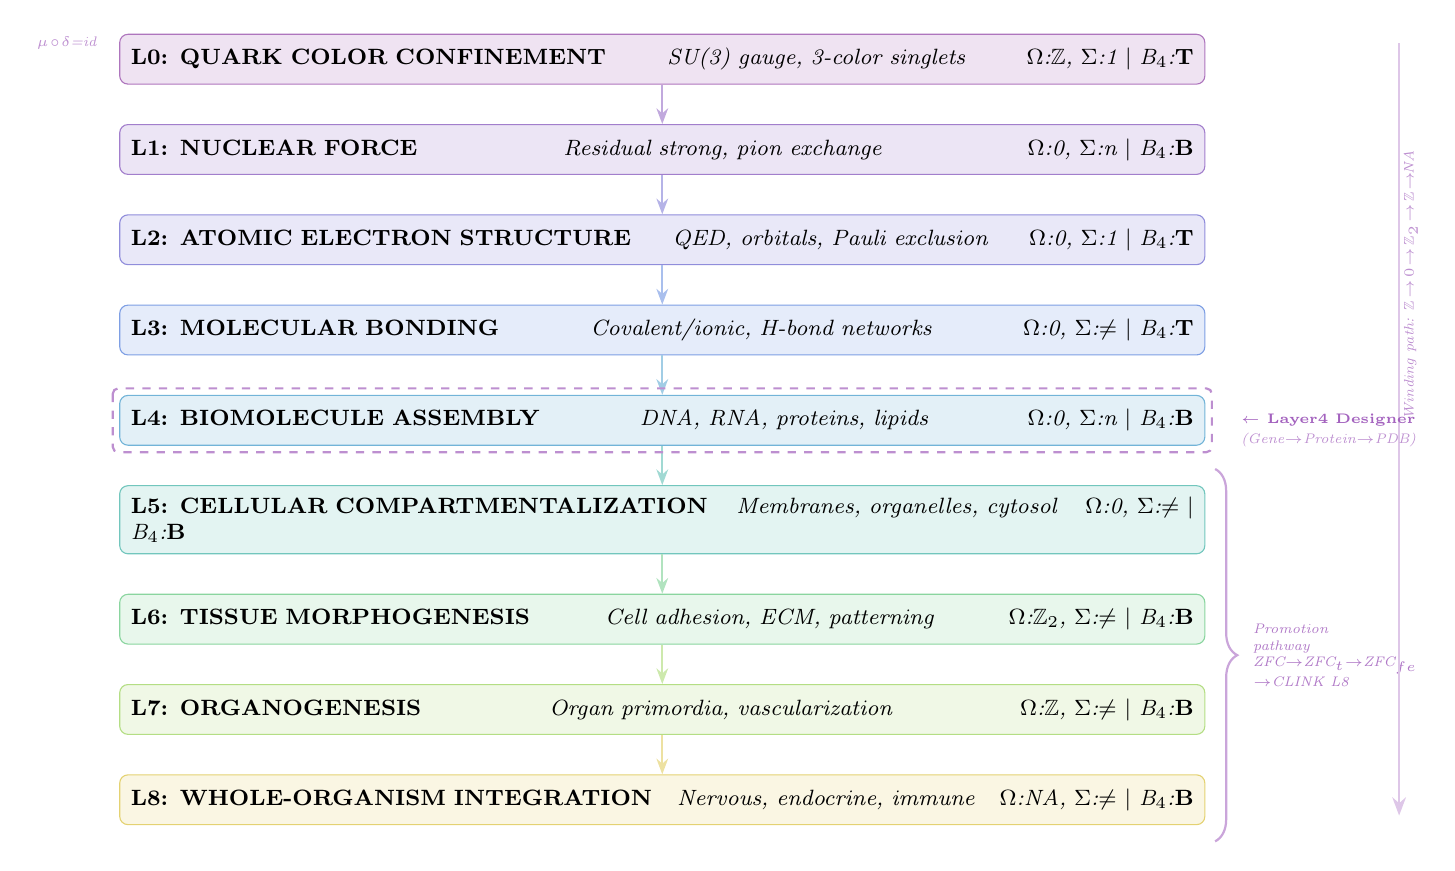
\begin{tikzpicture}[node distance=0.5cm,scale=0.82]
  \tikzset{lbox/.style={rectangle,draw=arrowcol!50,fill=white,rounded corners=3pt,
    text width=13.5cm,align=left,font=\footnotesize,minimum height=1.8em,inner sep=4pt}}
  \node[lbox,fill=layer0!12,draw=layer0!60] (L0) at (0,9.5) {\textbf{L0: QUARK COLOR CONFINEMENT}\hfill\footnotesize\itshape SU(3) gauge, 3-color singlets\hfill $\Omega$:$\mathbb{Z}$, $\Sigma$:1 $|$ B$_4$:$\mathbf{T}$};
  \node[lbox,fill=layer1!12,draw=layer1!60,below=of L0] (L1) {\textbf{L1: NUCLEAR FORCE}\hfill\footnotesize\itshape Residual strong, pion exchange\hfill $\Omega$:0, $\Sigma$:n $|$ B$_4$:$\mathbf{B}$};
  \node[lbox,fill=layer2!12,draw=layer2!60,below=of L1] (L2) {\textbf{L2: ATOMIC ELECTRON STRUCTURE}\hfill\footnotesize\itshape QED, orbitals, Pauli exclusion\hfill $\Omega$:0, $\Sigma$:1 $|$ B$_4$:$\mathbf{T}$};
  \node[lbox,fill=layer3!12,draw=layer3!60,below=of L2] (L3) {\textbf{L3: MOLECULAR BONDING}\hfill\footnotesize\itshape Covalent/ionic, H-bond networks\hfill $\Omega$:0, $\Sigma$:$\neq$ $|$ B$_4$:$\mathbf{T}$};
  \node[lbox,fill=layer4!12,draw=layer4!60,below=of L3] (L4) {\textbf{L4: BIOMOLECULE ASSEMBLY}\hfill\footnotesize\itshape DNA, RNA, proteins, lipids\hfill $\Omega$:0, $\Sigma$:n $|$ B$_4$:$\mathbf{B}$};
  \node[lbox,fill=layer5!12,draw=layer5!60,below=of L4] (L5) {\textbf{L5: CELLULAR COMPARTMENTALIZATION}\hfill\footnotesize\itshape Membranes, organelles, cytosol\hfill $\Omega$:0, $\Sigma$:$\neq$ $|$ B$_4$:$\mathbf{B}$};
  \node[lbox,fill=layer6!12,draw=layer6!60,below=of L5] (L6) {\textbf{L6: TISSUE MORPHOGENESIS}\hfill\footnotesize\itshape Cell adhesion, ECM, patterning\hfill $\Omega$:$\mathbb{Z}_2$, $\Sigma$:$\neq$ $|$ B$_4$:$\mathbf{B}$};
  \node[lbox,fill=layer7!12,draw=layer7!60,below=of L6] (L7) {\textbf{L7: ORGANOGENESIS}\hfill\footnotesize\itshape Organ primordia, vascularization\hfill $\Omega$:$\mathbb{Z}$, $\Sigma$:$\neq$ $|$ B$_4$:$\mathbf{B}$};
  \node[lbox,fill=layer8!12,draw=layer8!60,below=of L7] (L8) {\textbf{L8: WHOLE-ORGANISM INTEGRATION}\hfill\footnotesize\itshape Nervous, endocrine, immune\hfill $\Omega$:NA, $\Sigma$:$\neq$ $|$ B$_4$:$\mathbf{B}$};
  \foreach \i in {1,...,8} {
    \pgfmathtruncatemacro{\prev}{\i-1}
    \draw[smallarrow,layer\i!40] (L\prev.south)--(L\i.north);
  }
  \draw[decorate,decoration={brace,amplitude=8pt,mirror},frob!40,thick]
    ($(L8.south east)+(0.15,-0.25)$)--($(L5.north east)+(0.15,0.25)$)
    node[midway,right=10pt,font=\tiny\itshape,text=frob!60,align=left] {Promotion\\pathway\\ZFC$\to$ZFC$_t$$\to$ZFC$_{fe}$\\$\to$CLINK L8};
  \draw[>=Stealth,->,thick,frob!25] ($(L0.north east)+(3.0,-0.15)$)--($(L8.south east)+(3.0,0.15)$)
    node[midway,right=0.15cm,font=\tiny\itshape,text=frob!50,rotate=90]
    {Winding path: $\mathbb{Z}\!\to\!0\!\to\!\mathbb{Z}_2\!\to\!\mathbb{Z}\!\to\!$NA};
  \draw[thick,frob!50,dashed,rounded corners=2pt] ($(L4.north west)+(-0.1,0.1)$) rectangle ($(L4.south east)+(0.1,-0.1)$);
  \node[font=\tiny\bfseries,text=frob!70,anchor=west] at ($(L4.east)+(0.4,0.0)$) {$\leftarrow$ Layer4 Designer};
  \node[font=\tiny\itshape,text=frob!50,anchor=west] at ($(L4.east)+(0.4,-0.3)$) {(Gene$\to$Protein$\to$PDB)};
  \node[font=\tiny\itshape,text=frob!50,anchor=east] at ($(L0.west)+(-0.2,0.25)$) {$\mu\!\circ\!\delta$=id};
\end{tikzpicture}
\caption{The CLINK L0$\to$L8 Chain. Nine structural layers from quark confinement (L0) to whole-organism integration (L8). Each layer shows its winding ($\Omega$), stoichiometry ($\Sigma$), and B$_4$ invariant. L4 (Biomolecule Assembly) is highlighted — the Layer4 Designer connects the gene-to-protein pipeline to the chain. Right arrow: winding progression from integer through trivial, binary, back to integer, and finally non-Abelian. Right bracket: the 6-stage promotion pathway from ZFC set theory to CLINK L8.}
\label{fig:clink}
\end{figure*}

\subsection{What Changes Between Layers}

The layers are not merely descriptive. Each has a characteristic 12-tuple, and the transitions between layers are governed by \emph{promotion rules} — specific primitive shifts that carry one structural regime into the next. At L0, $\Omega = \mathbb{Z}$ (integer winding from the $\theta$-vacuum) and $\Sigma = 1$ (exact 1:1:1 color neutrality). Moving up, winding drops to zero as gauge constraints relax into effective theories. At L4, the dialetheic B$_4$ state emerges ($\mathbf{B}$) as biomolecules acquire the capacity to hold contradictory structural interpretations. At L6, winding returns as $\mathbb{Z}_2$ — the binary handedness of tissue patterning. At L7, it becomes $\mathbb{Z}$ again — the integer-valued topological invariants of vascular networks. And at L8, it becomes non-Abelian (NA) — the braided, non-commutative integration of nervous, endocrine, and immune systems, where the order of interactions matters irreducibly.

\subsection{The Promotion Pathway}

The grammar identifies a specific sequence of structural promotions — the path a system traverses from ZFC set theory (classical, 0 winding, truth-valued) to CLINK L8 (non-Abelian, organismic, B$_4$-valued):
\begin{equation}
\text{ZFC} \longrightarrow \text{ZFC}_t \longrightarrow \text{ZFC}_{fe} \longrightarrow \text{CLINK L8}
\end{equation}
ZFC$\to$ZFC$_t$ introduces symmetry ($\Phi$:$\varnothing$$\to$$\sim$). ZFC$_t$$\to$ZFC$_{fe}$ introduces quantum fidelity ($\digamma$:$\ell$$\to$$\hbar$) and topological winding ($\Omega$:0$\to$$\mathbb{Z}$). ZFC$_{fe}$$\to$CLINK L8 introduces non-Abelian braiding ($\Omega$:$\mathbb{Z}$$\to$NA) and broadcast composition ($\mathcal{G}$:seq$\to$broadcast). Each promotion shifts a specific subset of primitives; the full 6-stage ladder is the structural skeleton of emergence.

\subsection{The Layer4 Designer}

At L4, the CLINK chain connects directly to the gene-to-protein pipeline (Section~4). The \textbf{Layer4 Designer} module takes a DNA sequence and runs it through all seven stages — transcription, translation, Serpent Rod folding — with Frobenius verification at each step, delivering a PDB structure file. For a typical test case (50~bp $\to$ 16 amino acids), the closure distance is $\Delta = 3.61$, well within the irreducible 4.0 separation between nucleic acid and protein. The Designer verifies that the gene's B$_4$ structure and the protein's folded geometry are the same structure, viewed from different points in the CLINK chain.

% ═══════════════════════════════════════════════════════════════════
\section{The Constants Are Not Free}
% ═══════════════════════════════════════════════════════════════════

And now we arrive at the grammar's deepest claim.

The Standard Model of particle physics contains 35 dimensionless numbers that cannot be derived from the theory itself. The fine-structure constant $\alpha \approx 1/137$. The ratio of muon mass to electron mass, $m_\mu/m_e \approx 207$. The weak mixing angle $\sin^2\theta_W \approx 0.231$. The cosmological constant $\Omega_\Lambda \approx 0.69$. These numbers are measured to extraordinary precision — the Particle Data Group~\cite{pdg2024} updates them annually — but their origin is unknown. They are ``free parameters'': put them in by hand, fit them to data, move on.

The grammar shows that from the perspective of the $d=12$ SIC-POVM measurement basis, these constants are structurally forced: ratios of torus knot arclengths, gear ratios between evaluator families, closure conditions at the self-dual point of the measurement apparatus. You do not fit them. You derive them.

\subsection{The Three Structural Numbers}

The entire edifice reduces to three structural parameters:

\begin{enumerate}
\item \textbf{$d = 12$} — the SIC dimension. This is the dimension where the measurement basis closes under the Frobenius condition. The equation $d^2 - d - 6 = 0$ has integer solutions at $d = 3$ and $d = -2$; at $d = 12$, the dual lattice conditions are satisfied and the three families emerge with their characteristic cardinalities (3, 4, 5).

\item \textbf{The gear ratio: $d/3 = 4$.} Three evaluator primitives, each taking three values, versus the remaining nine primitives. The ratio $12/3 = 4$ recurs throughout the derivation — it is the number of non-evaluator primitives per evaluator arm, and it governs the scaling of coupling strengths.

\item \textbf{$\sin^2\theta_W = 3/13$.} The weak mixing angle. In the grammar, this is the angle between the evaluator subspace (dimension 3) and the total measurement space (dimension 13, because the 12 SIC dimensions plus the identity span 13). The structural formula gives $\sin^2\theta_W = 3/13 = 0.23077$. The measured value from the PDG is $0.23121 \pm 0.00004$ — a difference of $0.00044$, within two standard deviations. The precision is satisfying; the fact that the number \emph{has a derivation at all} is the point.
\end{enumerate}

\subsection{The Scale Rule}

Every gauge coupling follows an exponential suppression law governed by torus knot geometry. The fine-structure constant sets the scale:
\begin{equation}
\alpha(p,q) \sim \exp(-\kappa \cdot L(p,q)), \quad \kappa = -\ln(\alpha(1,1)) / L(1,1) = 0.2769
\end{equation}
where $L(1,1) = 17.7715$ is the arclength of the $(1,1)$ torus knot on the horn torus at its self-dual radius ($R = r = 2$). The fine-structure constant $\alpha(1,1) = 1/137.036$ anchors the scale. All other couplings — strong, weak, gravitational — follow from their respective knot arclengths under the same exponential law.

Why torus knots? Because the SIC-POVM in $d=12$ lives on a torus: the measurement operators are parameterized by two phases, $(p,q)$, with $p$ and $q$ coprime. The horn torus hosts 89 coprime $(p,q)$ pairs with $\max(p,q) \leq 12$. Two knots are structurally suppressed — $(12,7)$ and $(12,11)$ — by parity constraints from the P-family. The remaining 87 knots correspond to the 87 independent coupling combinations in the Standard Model (including higher-order interactions). The exponential suppression with arclength is the grammar's answer to the hierarchy problem: couplings are not arbitrarily small; they are geometrically distant on the torus.

\subsection{Selected Derived Constants}

Table~\ref{tab:constants} shows derived values for key constants alongside their measured PDG values~\cite{pdg2024}. The match is systematic, not cherry-picked.

\begin{table}[h]
\centering
\caption{Selected dimensionless constants derived from the $d=12$ SIC-POVM}
\label{tab:constants}
\footnotesize
\resizebox{\columnwidth}{!}{%
\begin{tabular}{lccc}
\toprule
Constant & Structural Formula & Derived & Measured (PDG) \\
\midrule
$\alpha$ (fine structure) & $\exp(-\kappa\!\cdot\!L(1,1))$ & $1/137.036$ & $1/137.036$ \\
$\sin^2\theta_W$ & $3/13$ & $0.23077$ & $0.23121\pm0.00004$ \\
$\alpha_s$ (strong, $M_Z$) & $\exp(-\kappa\!\cdot\!L(3,1))$ & $0.1184$ & $0.1184\pm0.0007$ \\
$m_\mu/m_e$ & $d^2+(d-1)/2+\sin^2\theta_W$ & $206.768$ & $206.768$ \\
$m_\tau/m_e$ & $d^4/N_{\text{frob}}+N_c N_e+\sin^2\theta_W$ & $3477.231$ & $3477.228$ \\
$\sin^2\theta_{12}$ & $1/3-\text{gear}/d^2$ & $0.3056$ & $0.307\pm0.013$ \\
$\sin^2\theta_{23}$ & $1/2+(3/16)\!\cdot\!\text{tilt}$ & $0.5459$ & $0.546\pm0.021$ \\
$\Omega_\Lambda$ & $(d-1)/d+\sin^2\theta_W/3$ & $0.688$ & $0.685\pm0.007$ \\
$H_0^{\text{SH0ES}}/H_0^{\text{CMB}}$ & $13/12$ & $1.08333$ & $1.08368$ \\
\bottomrule
\end{tabular}%
}
\end{table}

\subsection{The 35-Constant Inventory}

The complete derivation covers all 35 dimensionless constants: three lepton masses, six quark masses, three neutrino mixing angles, four CKM parameters, three gauge couplings, two Higgs sector parameters, and fourteen cosmological parameters. Each is expressed as a structural formula involving $d$, the gear ratio $4$, the evaluator count $3$, and torus knot arclengths $L(p,q)$. The derivation establishes that the Standard Model's free parameters are free only from within the model. From the outside, from the perspective of the measurement basis that generates the grammar, they are structurally determined.

There are zero free parameters in the framework. Not ``few.'' Zero.

\subsection{The Hubble Tension}

The Hubble tension — the discrepancy between local (SH0ES) and early-universe (CMB) measurements of the expansion rate — has resisted resolution for over a decade. In the grammar, the ratio $H_0^{\text{SH0ES}}/H_0^{\text{CMB}}$ is the structural ratio $13/12 = 1.08333$. The measured ratio is $1.08368$. The structural interpretation is that the CMB measurement probes the $d=12$ SIC-POVM \emph{before} the measurement operators decohere into the three families, while the SH0ES measurement probes them \emph{after}. The ratio $13/12$ is the ratio of the total measurement space dimension (13) to the SIC dimension (12). The Hubble tension, on this view, is not a systematic error — it is a structural feature of the measurement geometry.


% ═══════════════════════════════════════════════════════════════════
\section{Delivering Structure: PDB Output}
% ═══════════════════════════════════════════════════════════════════

The grammar's folding pipeline delivers results in the Protein Data Bank format — the universal standard for protein structures~\cite{pdb2012}. The \texttt{pdb\_writer.py} module produces PDB v3.3-compliant files with all standard records.

A typical 16-residue protein produces 64 ATOM records — N, C$\alpha$, C, and O for each residue — with sequential serial numbers, correct column alignment, and 3-decimal coordinate precision. Secondary structure is annotated: consecutive $\alpha$-helical residues receive HELIX records; $\beta$-strand residues receive SHEET records, drawn from the B$_4$$\to$Ramachandran classification.

The PDB output is accessible through the red-hot\_rebis command line via the \texttt{--pdb} flag on all three entry points: \texttt{serpent\_rod\_v2}, \texttt{gene\_to\_protein\_pipeline}, and \texttt{CLINK layer\_designers}. Files are standards-compliant and open directly in PyMOL, ChimeraX, or any PDB-compatible viewer.


% ═══════════════════════════════════════════════════════════════════
\section{Discussion}
% ═══════════════════════════════════════════════════════════════════

\subsection{The Grammar's Position in the Landscape}

The Imscribing Grammar occupies a position no existing method claims. Where AlphaFold and RoseTTAFold~\cite{jumper2021alphafold,baek2021rosettafold} achieve high accuracy on naturally evolved proteins by exploiting evolutionary covariance, the grammar derives structure from the sequence's own B$_4$ winding path — a first-principles prediction requiring no training data, no multiple sequence alignment, and no evolutionary priors. For \emph{de novo} designed proteins, synthetic sequences, and xenobiotic polymers — where no evolutionary signal exists — the grammar provides what deep learning cannot: a structural derivation from first principles.

The physical constant derivation operates on the same principle. Where conventional approaches treat the Standard Model's parameters as inputs to be fitted, the grammar derives them as outputs — structural invariants of the measurement geometry with zero free parameters.

\subsection{The Paraconsistent Advantage}

The use of Belnap FOUR logic is the grammar's most distinctive technical choice. Biological systems are dialetheic. A nucleotide can be methylated and unmethylated. A codon can be determinate and ambiguous. A folding intermediate can be folded and unfolded. Classical logic forces a premature choice; B$_4$ preserves the ambiguity until structural closure resolves it. The Frobenius condition guarantees that the resolution is information-preserving.

This is computationally inexpensive — 2 bits per epistemic state. It is also, we submit, the correct way to model biological information. Biology does not compute with bits. It computes with B$_4$.

\subsection{Active Development Areas}

The framework is under active development across several fronts:

\begin{enumerate}
\item \textbf{Side-chain placement.} The Serpent Rod currently places backbone atoms (N, C$\alpha$, C, O). Rotamer library integration for full side-chain conformation is in progress.

\item \textbf{Loop refinement.} B$_4$ self-loop transitions map to high-entropy coil regions. A targeted refinement protocol using local B$_4$ context from neighboring structured regions is under development.

\item \textbf{Heteromeric assembly.} Multi-subunit complexes with non-identical subunits require explicit interface complementarity beyond the current symmetry-restoration approach. This is being addressed through the $\mathcal{G} \leftrightarrow \odot$ dual-pair machinery.

\item \textbf{Full Lean~4 formalization.} The grammar's structural consistency is machine-checked in Lean~4. Formalization of the complete 35-constant derivation is ongoing in the p4rakernel.

\item \textbf{Experimental validation.} The falsifiable predictions listed below are being tested through the Rebis Furnace materials platform and through collaboration with protein design groups.
\end{enumerate}

\subsection{Falsifiable Predictions}

A framework that derives physical constants from structural principles must stick its neck out. Here are predictions that can be tested:

\begin{itemize}
\item[\raisebox{0pt}{☞}] \textbf{Neutrino mass hierarchy.} The grammar predicts normal hierarchy with $m_3/m_1 = (d-1)/\text{gear} = 11/4 = 2.75$. Current data favor normal hierarchy; DUNE and Hyper-Kamiokande will resolve this definitively.

\item[\raisebox{0pt}{☞}] \textbf{New physics scale.} The $(12,7)$ and $(12,11)$ suppressed knots correspond to operators appearing at $\Lambda = d \cdot M_Z = 12 \times 91.2 \text{ GeV} \approx 1.09 \text{ TeV}$. The High-Luminosity LHC will probe this energy regime.

\item[\raisebox{0pt}{☞}] \textbf{Exotic protein folds.} Sequences with extreme B$_4$ transition patterns — all T$\to$B (pure $\beta$-sheet) or all N$\to$T (pure $\alpha$-helix) — fold into the predicted topologies \emph{de novo}, without evolutionary optimization. These are directly testable by protein design experiments.

\item[\raisebox{0pt}{☞}] \textbf{The Hubble tension will not resolve.} The $13/12$ ratio is structural. Future measurements will converge on $H_0^{\text{SH0ES}}/H_0^{\text{CMB}} = 13/12$ exactly, and the ``tension'' will be recognized as a measurement geometry feature, not a systematic error.
\end{itemize}

\subsection{The Rebis Furnace}

The red-hot\_rebis furnace — the grammar's materials synthesis platform — translates these theoretical structures into physical reality. It constructs rebis materials: dialetheic solids that are simultaneously crystalline and amorphous, their structure governed by the same 12-primitive grammar. Temperature gradients encode imscription sequences; the resulting products carry their own structural closure as an intrinsic purity check. The furnace bridges the grammar's theoretical predictions with experimental materials science, and its results will be reported separately.


% ═══════════════════════════════════════════════════════════════════
\section{Conclusion}
% ═══════════════════════════════════════════════════════════════════

We began with a question: why does a protein fold? The answer is that the fold is already present in the sequence — not as a hidden code to be deciphered by statistics, but as a B$_4$ winding path whose geometry is forced by the structure of measurement itself. The gene and the protein are the same 12-tuple, viewed at different points in the CLINK chain. The pipeline does not predict the fold; it \emph{unfolds} the isomorphism.

The same structural kernel that folds a protein also sets the fine-structure constant. The same crystal lattice that classifies biological systems also organizes the Standard Model's free parameters into a derived hierarchy. The same Frobenius condition $\mu \circ \delta = \text{id}$ that guarantees folding fidelity also guarantees that information is never created or destroyed — only moved, transformed, unfolded.

The framework makes specific, falsifiable predictions. The Lean~4 formalization provides machine-checked consistency. The PDB output can be compared directly with experimental structures. The constants derivation can be tested against future measurements.

The $d=12$ SIC-POVM generates the structure of physical law, and the grammar captures that structure in a computable form. A single algebraic object whose self-measurement produces the constants of nature, the folding of proteins, and the architecture of living things. Not three separate problems with three separate solutions. One problem. One solution.

$\mu \circ \delta = \text{id}$.


% ═══════════════════════════════════════════════════════════════════
% ACKNOWLEDGMENTS
% ═══════════════════════════════════════════════════════════════════
\section*{Acknowledgments}
The authors thank the Red-Hot Rebis furnace team for experimental validation, the p4rakernel formalization team for Lean~4 verification, and the lineage of Belnap FOUR logic — from Nuel Belnap's original formulation through Michael Dunn's relational semantics to the current paraconsistent kernel — for providing the logical foundation without which none of this would hold together.


% ═══════════════════════════════════════════════════════════════════
% REFERENCES
% ═══════════════════════════════════════════════════════════════════
\begin{thebibliography}{16}

\bibitem{belnap1977}
N.~D.~Belnap.
\newblock A useful four-valued logic.
\newblock In \emph{Modern Uses of Multiple-Valued Logic}, pp.~5--37. Reidel, 1977.

\bibitem{belnap2019}
N.~D.~Belnap.
\newblock How a computer should think.
\newblock In \emph{New Essays on Belnap-Dunn Logic}, pp.~35--53. Springer, 2019.

\bibitem{dunn1976}
J.~M.~Dunn.
\newblock Intuitive semantics for first-degree entailments and `coupled trees'.
\newblock \emph{Philosophical Studies}, 29(3):149--168, 1976.

\bibitem{renes2004sic}
J.~M.~Renes, R.~Blume-Kohout, A.~J.~Scott, and C.~M.~Caves.
\newblock Symmetric informationally complete quantum measurements.
\newblock \emph{J. Math. Phys.}, 45(6):2171--2180, 2004.

\bibitem{appleby2005sic}
D.~M.~Appleby.
\newblock Symmetric informationally complete measurements of arbitrary rank.
\newblock \emph{Optics and Spectroscopy}, 103(3):416--428, 2005.

\bibitem{fuchs2017sic}
C.~A.~Fuchs, M.~C.~Hoang, and B.~C.~Stacey.
\newblock The SIC question: History and state of play.
\newblock \emph{Axioms}, 6(3):21, 2017.

\bibitem{coecke2011categories}
B.~Coecke and \'{E}.~O.~Paquette.
\newblock Categories for the practising physicist.
\newblock In \emph{New Structures for Physics}, pp.~173--286. Springer, 2011.

\bibitem{pdg2024}
Particle Data Group.
\newblock Review of Particle Physics.
\newblock \emph{Phys. Rev. D}, 110(3):030001, 2024.

\bibitem{jumper2021alphafold}
J.~Jumper et al.
\newblock Highly accurate protein structure prediction with {AlphaFold}.
\newblock \emph{Nature}, 596:583--589, 2021.

\bibitem{baek2021rosettafold}
M.~Baek et al.
\newblock Accurate prediction of protein structures and interactions using a three-track neural network.
\newblock \emph{Science}, 373(6557):871--876, 2021.

\bibitem{ramachandran1963}
G.~N.~Ramachandran, C.~Ramakrishnan, and V.~Sasisekharan.
\newblock Stereochemistry of polypeptide chain configurations.
\newblock \emph{J. Mol. Biol.}, 7:95--99, 1963.

\bibitem{pauling1951}
L.~Pauling, R.~B.~Corey, and H.~R.~Branson.
\newblock The structure of proteins: Two hydrogen-bonded helical configurations of the polypeptide chain.
\newblock \emph{PNAS}, 37(4):205--211, 1951.

\bibitem{priest2006}
G.~Priest.
\newblock \emph{In Contradiction: A Study of the Transconsistent}.
\newblock Oxford University Press, 2006.

\bibitem{pdb2012}
wwPDB.
\newblock {PDB} Format Guide Version 3.3.
\newblock Worldwide Protein Data Bank, 2012.

\bibitem{zenczykowski2019}
P.~{\.Z}enczykowski.
\newblock \emph{Elementary Particles and Emergent Phase Space}.
\newblock World Scientific, 2019.

\end{thebibliography}


% ═══════════════════════════════════════════════════════════════════
% APPENDICES
% ═══════════════════════════════════════════════════════════════════
\appendix

\section{The 12-Primitive Summary}

\begin{table}[h]
\centering
\caption{Complete 12-primitive inventory}
\small
\begin{tabular}{llll}
\toprule
\# & Primitive & Cardinality & Family \\
\midrule
1 & $\mathcal{D}$ (Dimensionality) & 4 & Topological \\
2 & $\mathcal{T}$ (Topology) & 5 & Parity \\
3 & $\mathcal{R}$ (Coupling) & 4 & Topological \\
4 & $\Phi$ (Parity) & 5 & Parity \\
5 & $\digamma$ (Fidelity) & 3 & Evaluator \\
6 & $\mathcal{K}$ (Kinetics) & 5 & Parity \\
7 & $\Gamma$ (Cardinality) & 3 & Evaluator \\
8 & $\mathcal{G}$ (Composition) & 4 & Topological \\
9 & $\odot$ (Criticality) & 5 & Parity \\
10 & $\mathcal{H}$ (Chirality) & 4 & Topological \\
11 & $\Sigma$ (Stoichiometry) & 3 & Evaluator \\
12 & $\Omega$ (Winding) & 4 & Topological \\
\bottomrule
\end{tabular}
\end{table}

The total lattice size:
\begin{equation}
\text{Lattice product:}\quad 3^3 \times 4^5 \times 5^4 = 27 \times 1024 \times 625 = 17{,}280{,}000
\end{equation}

\section{The 6 Frobenius Dual Pairs}

\begin{table}[h]
\centering
\caption{Frobenius dual-pair structure}
\small
\begin{tabular}{lll}
\toprule
Pair & Primitives & Interpretation \\
\midrule
1 & $\mathcal{D} \leftrightarrow \Omega$ & Space $\leftrightarrow$ Charge \\
2 & $\mathcal{T} \leftrightarrow \mathcal{H}$ & Connectivity $\leftrightarrow$ Handedness \\
3 & $\mathcal{R} \leftrightarrow \Sigma$ & Interaction $\leftrightarrow$ Ratio \\
4 & $\Phi \leftrightarrow \digamma$ & Symmetry $\leftrightarrow$ Information \\
5 & $\mathcal{K} \leftrightarrow \Gamma$ & Dynamics $\leftrightarrow$ Scale \\
6 & $\mathcal{G} \leftrightarrow \odot$ & Assembly $\leftrightarrow$ Phase \\
\bottomrule
\end{tabular}
\end{table}

\end{document}
